
%%%%%%%%%%%%%%%%%%%%%%%%%%%%%%%%%%%%%%%%%%%%%%%%%%%%%%%%%%%%%%%%%%%%%%%%%%%%%%%%%%%%%%
%%%%%%%%%%%%%%%%%%%%%%%%%%%%%%%%%%%%%%%%%%%%%%%%%%%%%%%%%%%%%%%%%%%%%%%%%%%%%%%%%%%%%%
\section{Preserving the Privacy of User Data}
%%%%%%%%%%%%%%%%%%%%%%%%%%%%%%%%%%%%%%%%%%%%%%%%%%%%%%%%%%%%%%%%%%%%%%%%%%%%%%%%%%%%%%
%%%%%%%%%%%%%%%%%%%%%%%%%%%%%%%%%%%%%%%%%%%%%%%%%%%%%%%%%%%%%%%%%%%%%%%%%%%%%%%%%%%%%%
\label{sec:privacy}
% Editors: (Peter Kairouz, Kallista Bonawitz, Adria Gascon)

\begin{figure}[b!] 
% Uses the figure saved when this figure was originally presented in Section 1.
\noindent\usebox{\actorsfigure}
% Reuses the original figure number and calls out the page where this figure originally appeared.
\repeatcaption{fig:actors}{The lifecycle of an FL-trained model and the various actors in a federated learning system.
\label{fig:actors_repeat}
} 
\end{figure}


Machine learning workflows involve many actors functioning in disparate capacities.  For example, users may generate training data through interactions with their devices, a machine learning training procedure extracts cross-population patterns from this data (e.g. in the form of trained model parameters), the machine learning engineer or analyst may assess the quality of this trained model, and eventually the model may be deployed to end users in order to support specific user experiences (see Figure~\ref{fig:actors} below).  

In an ideal world, each actor in the system would learn nothing more than the information needed to play their role.  For example, if an analyst only needs to determine whether a particular quality metric exceeds a desired threshold in order to authorize deploying the model to end users, then in an idealized world, that is the only bit of information that would be available to the analyst; such an analyst would need access to neither the training data nor the model parameters, for instance.  Similarly, end users enjoying the user experiences powered by the trained model might only require predictions from the model and nothing else.

Furthermore, in an ideal world every participant in the system would be able to reason easily and accurately about what personal information about themselves and others might be revealed by their participation in the system, and participants would be able to use this understanding to make informed choices about how and whether to participate at all.

Producing a system with all of the above ideal privacy properties would be a daunting feat on its own, and even more so while also guaranteeing other desirable properties such as ease of use for all participants, the quality and fairness of the end user experiences (and the models that power them), the judicious use of communication and computation resources, resilience against attacks and failures, and so on.

Rather than allowing perfect to be the enemy of good, we advocate a strategy wherein the overall system is composed of modular units which can be studied and improved relatively independently, while also reminding ourselves that we must, in the end, measure the privacy properties of the complete system against our ideal privacy goals set out above. The open questions raised throughout this section will highlight areas wherein we do not yet understand how to simultaneously achieve all of our goals, either for an individual module or for the system as a whole.

Federated learning provides an attractive structure for decomposing the overall machine learning workflow into the approachable modular units we desire.  One of the primary attractions of the federated learning model is that it can provide a level of privacy to participating users through data minimization: the raw user data never leaves the device, and only updates to models (e.g., gradient updates) are sent to the central server. These model updates are more focused on the learning task at hand than is the raw data (i.e. they contain strictly no additional information about the user, and typically significantly less, compared to the raw data), and the individual updates only need to be held ephemerally by the server.  

While these features can offer significant practical privacy improvements over centralizing all the training data, there is still no formal guarantee of privacy in this baseline federated learning model. For instance, it is possible to construct scenarios in which information about the raw data is leaked from a client to the server, such as a scenario where knowing the previous model and the gradient update from a user would allow one to infer a training example held by that user. Therefore, this section surveys existing results and outlines open challenges towards designing federated learning systems that can offer rigorous privacy guarantees. We focus on questions specific to the federated learning and analytics setting and leave aside questions that also arise in more general machine learning settings as surveyed in \cite{pdlSurvey}.

Beyond attacks targeting user privacy, there are also other classes of attacks on federated learning; for example, an adversary might attempt to prevent a model from being learned at all, or they might attempt to bias the model to produce inferences that are preferable to the adversary.  We defer consideration of these types of attacks to Section~\ref{sec:robust}.

The remainder of this section is organized as follows. Section \ref{ssec:actors_threat_models} discusses various threat models against which we wish to give protections. Section \ref{ssec:tools_tech} lays out a set of core tools and technologies that can be used towards providing rigorous protections against the threat models discussed in Section \ref{ssec:actors_threat_models}. Section \ref{ssec:adv_clients_analysts} assumes the existence of a trusted server and discusses the open problems and challenges in providing protections against adversarial clients and/or analysts. Section \ref{ssec:adv_server} discusses the open problems and challenges in the absence of a fully trusted server. Finally, Section \ref{ssec:user_perception} discusses open questions around user perception. 

\subsection{Actors, Threat Models, and Privacy in Depth}
\label{ssec:actors_threat_models}

A formal treatment of privacy risks in FL calls for a holistic and interdisciplinary approach. While some of the risks can be mapped to technical privacy definitions and mitigated with existing technologies, others are more complex and require cross-disciplinary efforts. 

Privacy is not a binary quantity, or even a scalar one. This first step towards such formal treatment is a careful characterization of the different actors (see Figure \ref{fig:actors} from \cref{sec:intro}, repeated on page~\pageref{fig:actors_repeat} for convenience) and their roles to ultimately define relevant threat models (see Table \ref{table:actors_and_threats}). Thus, for instance, it is desirable to distinguish the view of the server administrator from the view of the analysts that consume the learned models, as it is conceivable that a system that is designed to offer strong privacy guarantees against a malicious analyst may not provide any guarantees with respect to a malicious server. These actors map well onto the threat models discussed elsewhere in the literature; for example, in \citet[Sec 3.1]{prochlo}, where the ``encoder'' corresponds to the client, the ``shuffler'' generally corresponds to the server, the ``analyzer`` may correspond to the server or post-processing done by the analyst.

As an example, a particular system might offer a differential privacy\footnote{Differential privacy will be formally introduced in Section \ref{sssec:private_disclosures}.  For now, it suffices to know that lower $\varepsilon$ corresponds with higher privacy.} guarantee with a particular parameter $\varepsilon$ to the view of the server administrator, while the results observed by analysts might have a higher protection $\varepsilon' < \varepsilon$. 

Furthermore, it is possible that this guarantee holds only against adversaries with particular limits on their capabilities, e.g. an adversary that can observe everything that happens on the server (but cannot influence the server's behavior) while simultaneously controlling up to a fraction $\gamma$ of the clients (observing everything they see and influencing their behavior in arbitrary ways); the adversary might also be assumed to be unable to break cryptographic mechanisms instantiated at a particular security level $\sigma$.  Against an adversary whose strength \textit{exceeds} these limits, the view of the server administrator might still have some differential privacy, but at weaker level $\varepsilon_0 > \varepsilon$.  

As we see in this example, precisely specifying the assumptions and privacy goals of a system can easily implicate concrete instantiations of several parameters ($\varepsilon, \varepsilon', \varepsilon_0, \gamma, \sigma$, etc.) as well as concepts such as differential privacy and honest-but-curious security.

\begin{table}
\renewcommand{\arraystretch}{1.2}
\begin{center} 
\begin{tabular}{@{}p{1.2in} p{1.85in}  p{3in}@{}}
\toprule
\textbf{Data/Access Point} & \textbf{Actor} & \textbf{Threat Model} \\
\midrule
\addlinespace[0.05in]
Clients & 
Someone who has root access to the client device, either by design or by compromising the device &
Malicious clients can inspect all messages received from the server (including the model iterates) in the rounds they participate in and can tamper with the training process.  An honest-but-curious client can inspect all messages received from the server but cannot tamper with the training process.   In some cases, technologies such as secure enclaves/TEEs may be able to limit the influence and visibility of such an attacker, representing a meaningfully weaker threat model.
\\ 
\addlinespace[0.1in]
%\hline
Server & 
Someone who has root access to the server, either by design or by compromising the device &
A malicious server can inspect all messages sent to the server (including the gradient updates) in all rounds and can tamper with the training process. An honest-but-curious server can inspect all messages sent to the server but cannot tamper with the training process.  In some cases, technologies such as secure enclaves/TEEs may be able to limit the influence and visibility of such an attacker, representing a meaningfully weaker threat model.
\\ 
\addlinespace[0.1in]
%\hline
Output Models &
Engineers \& analysts & 
A malicious analyst or model engineer may have access to multiple outputs from the system, e.g. sequences of model iterates from multiple training runs with different hyperparameters. Exactly what information is released to this actor is an important system design question. 
\\
\addlinespace[0.1in]
%\hline
Deployed Models &
The rest of the world & 
In cross-device FL, the final model may be deployed to hundreds of millions of devices. A partially compromised device can have black-box access to the learned model, and a fully compromised device can have a white-box access to the learned model.
\\ 
\addlinespace[0.05in]
\bottomrule
\end{tabular} 
\end{center}
\caption{Various threat models for different adversarial actors.} 
\label{table:actors_and_threats}
 \end{table}

% In addition to potentially adversarial individual actors, we often also need to consider collusions of adversaries, or adversaries with simultaneous influence over multiple actors in the system.  For example, a Secure Multi-Party Computation protocol running between the server and a cohort of clients might be secure against a multi-actor adversary with honest-but-curious access to the server and malicious control over a fraction of the participating clients.

Achieving all the desired privacy properties for federated learning will typically require composing many of the tools and technologies described below into an end-to-end system, potentially both layering multiple strategies to protect the same part of the system (e.g. running portions of a Secure Multi-Party Computation (MPC) protocol inside a Trusted Execution Environment (TEE) to make it harder for an adversary to sufficiently compromise that component) as well as using different strategies to protect different parts of the system (e.g. using MPC to protect the aggregation of model updates, then using Private Disclosure techniques before sharing the aggregate updates beyond the server).

As such, we advocate for building federated systems wherein the privacy properties degrade as gracefully as possible in cases where one technique or another fails to provide its intended privacy contribution.  For example, running the server component of an MPC protocol inside a TEE might allow privacy to be maintained even in the case where either (but not both) of the TEE security or MPC security assumptions fails to hold in practice.  As another example, requiring clients to send raw training examples to a server-side TEE would be strongly dispreferred to having clients send gradient updates to a server-side TEE, as the latter's privacy expectations degrade much more gracefully if the TEE's security were to fail.  We refer to this principle of graceful degradation as ``Privacy in Depth,’’ in analogy to the well-established network security principle of defense in depth \cite{nsa2012defense}.

\subsection{Tools and Technologies}
\label{ssec:tools_tech}
Generally speaking, the goal of an FL computation is for the analyst or engineer requesting the computation to obtain the result, which can be thought of as the evaluation of a function $f$ on a distributed client dataset (commonly an ML model training algorithm, but possibly something simpler such as a basic statistic). There are three privacy aspects that need to be addressed.

First, we need to consider {\em how} $f$ is computed and what is the information flow of intermediate results in the process, which primarily influences the susceptibility to malicious client, server, and admin actors.  In addition to designing the flow of information in the system (e.g. early data minimization), techniques from secure computation including Secure Multi-Party Computation (MPC) and Trusted Execution Environments (TEEs) are of particular relevance to addressing these concerns.  These technologies will be discussed in detail in \cref{sssec:secure_computations}.
% TODO(mcmahan): (Local) DP also has a role here, worth mentioning?

Second, we have to consider {\em what} is computed. In other words, how much information about a participating client is revealed to the analyst and world actors by the result of $f$ itself. Here, techniques for privacy-preserving disclosure, particularly differential privacy (DP), are highly relevant and will be discussed in detail in \cref{sssec:private_disclosures}.

Finally, there is the problem of {\em verifiability}, which pertains to the ability of a client or the server to prove to others in the system that they have executed the desired behavior faithfully, without revealing the potentially private data upon which they were acting.  Techniques for verifiability, including remote attestation and zero-knowledge proofs, will be discussed in \cref{sssec:verifiability}.

\begin{table}
\renewcommand{\arraystretch}{1.2}
\begin{center} 
\begin{tabular}{@{}p{2in} p{4in}@{}}
 \toprule 
\textbf{Technology} & \textbf{Characteristics} \\
\midrule
\addlinespace[0.05in]
Differential Privacy (local, central, shuffled, aggregated, and hybrid models) & A quantification of how much information could be learned about an individual from the output of an analysis on a dataset that includes the user. Algorithms with differential privacy necessarily incorporate some amount of randomness or noise, which can be tuned to mask the influence of the user on the output. 
\\
\addlinespace[0.1in]
%\hline
Secure Multi-Party Computation & Two or more participants collaborate to simulate, though cryptography, a fully trusted third party who can:
\begin{itemize} 
\item  Compute a function of inputs provided by all the participants;
\item Reveal the computed value to a chosen subset of the participants, with no party learning anything further.
\end{itemize}
\\
\addlinespace[0.1in]
%\hline
Homomorphic Encryption & Enables a party to compute functions of data to which they do not have plain-text access, by allowing mathematical operations to be performed on ciphertexts without decrypting them.  Arbitrarily complicated functions of the data can be computed this way (``Fully Homomorphic Encryption’’) though at greater computational cost. 
\\
\addlinespace[0.1in]
%\hline
Trusted Execution Environments (secure enclaves) & TEEs provide the ability to trustably run code on a remote machine, even if you do not trust the machine's owner/administrator.  This is achieved by limiting the capabilities of any party, including the administrator.  In particular, TEEs may provide the following properties \cite{subramanyan2017formal}:
\begin{itemize}
\item Confidentiality: The state of the code's execution remains secret, unless the code explicitly publishes a message;
\item Integrity: The code's execution cannot be affected, except by the code explicitly receiving an input;
\item Measurement/Attestation: The TEE can prove to a remote party what code (binary) is executing and what its starting state was, defining the initial conditions for confidentiality and integrity.
\end{itemize}
\\
\addlinespace[0.05in] 
\bottomrule
\end{tabular} 
\end{center}
\caption{Various technologies along with their characteristics.} 
\label{table:technologies}
\end{table}

\subsubsection{Secure Computations}
\label{sssec:secure_computations}

The goal of secure computation is to evaluate functions on distributed inputs in a way that only reveals the result of the computation to the intended parties, without revealing any additional information (e.g. the parties' inputs or any intermediate results). 

\paragraph{Secure multi-party computation}

Secure Multi-Party Computation (MPC) is a subfield of cryptography concerned with the problem of having a set of parties compute an agreed-upon function of their private inputs in a way that only reveals the intended output to each of the parties. This area was kicked off in the 1980’s by Yao~\cite{DBLP:conf/focs/Yao86}.  Thanks to both theoretical and engineering breakthroughs, the field has moved from being of a purely theoretical interest to a deployed technology in industry~\cite{DBLP:conf/fc/BogetoftCDGJKNNNPST09,DBLP:conf/fc/BogdanovTW12,DBLP:conf/secdev/LapetsVBJV16,araki2016high,DBLP:conf/eurocrypt/FurukawaLNW17,DBLP:journals/iacr/IonKNPSSSY17,DBLP:journals/iacr/IonKNPRSSSY19}. It is important to remark that MPC defines a set of technologies, and should be regarded more as a field, or a general notion of security in secure computation, than a technology \textit{per se}. Some of the recent advances in MPC can be attributed to breakthroughs in lower level primitives, such as oblivious transfer protocols~\cite{IKNP} and encryption schemes with homomorphic properties (as described below). 

A common aspect of cryptographic solutions is that operations are often done on a finite field (e.g. integers modulo a prime $p$), which poses difficulties when representing real numbers. A common approach has been to adapt ML models and their training procedures to ensure that (over)underflows are controlled, by operating on normalized quantities and relying on careful quantization~\cite{GasconSB0DZE17, quotient, gbdllnwCN, DBLP:conf/crypto/BourseMMP18}.

It has been known for several decades that any function can be securely computed, even in the presence of malicious adversaries~\cite{goldreich87}.
While generic solutions exist, their performance characteristics often render them inapplicable in practical settings.  As such a noticeable trend in research has consisted in designing custom protocols for applications such as linear and logistic regression~\cite{DBLP:conf/sp/NikolaenkoWIJBT13,GasconSB0DZE17, secureml} and neural network training and inference~\cite{secureml, quotient, bedkSE}. These works are typically in the cross-silo setting, or the variant where computation is delegated to a small group of computing servers that do not collude with each other. Porting these protocols to the cross-device setting is not straightforward, as they require a significant amount of communication.

\subparagraph{Homomorphic encryption}
Homomorphic encryption (HE) schemes allow certain mathematical operations to be performed directly on ciphertexts, without prior decryption.  Homomorphic encryption can be a powerful tool for enabling MPC by enabling a participant to compute functions on values while keeping the values hidden.

Different flavours of HE exist, ranging from general fully homomorphic encryption (FHE)~\cite{gentry2009fully} to the more efficient leveled variants~\cite{BFV1, BFV2, BGV, DBLP:conf/pkc/CoronLT14}, for which several implementations exist~\cite{HElib, SEAL, Palisade, SHELL, lattigo}. Also of practical relevance are the so-called partially homomorphic schemes, including for example ElGamal and Paillier, allowing either homomorphic addition or multiplication. Additive HE has been used as an ingredient in MPC protocols in the cross-silo setting~\cite{DBLP:conf/sp/NikolaenkoWIJBT13, Hardy2017-da}.
A review of some homomorphic encryption software libraries along with brief explanations of criteria/features to be considered in choosing a library is surveyed in \cite{sathya2018review}.\par
When considering the use of HE in the FL setting, questions immediately arise about
who holds the secret key of the scheme. While the idea of every client encrypting 
their data and sending it to the server to compute homomorphically 
on it is appealing, the server should not be able to decrypt a single client contribution.
A trivial way of overcoming this issue would be relying on a non-colluding external
party that holds the secret key and decrypts the result of the computation.
However, most HE schemes require that the secret keys be renewed often (due to e.g. susceptibility to chosen ciphertext attacks~\cite{DBLP:conf/latincrypt/ChenalT14}). Moreover, the availability of a trusted non-colluding 
party is not standard in the FL setting. 

Another way around this issue is relying on distributed (or threshold) encryption schemes, where the secret key is distributed among the parties. \citet{hatelove} and \citet{DBLP:conf/sosp/RothNFH19} propose such solutions for computing summation in the cross-device setting. Their protocols make use of additively homomorphic schemes (variants of ElGamal and lattice-based schemes, respectively).

\paragraph{Trusted execution environments}
Trusted execution environments (TEEs, also referred to as secure enclaves) may provide opportunities to move part of the federated learning process into a trusted environment in the cloud, whose code can be attested and verified.

TEEs can provide several crucial facilities for establishing trust that a unit of code has been executed faithfully and privately~\cite{subramanyan2017formal}:
\begin{itemize}
\item Confidentiality: The state of the code's execution remains secret, unless the code explicitly publishes a message.
\item Integrity: The code's execution cannot be affected, except by the code explicitly receiving an input.
\item Measurement/Attestation: The TEE can prove to a remote party what code (binary) is executing and what its starting state was, defining the initial conditions for confidentiality and integrity.
\end{itemize}

TEEs have been instantiated in many forms, including Intel's SGX-enabled CPUs~\cite{intel2012architecture,costan2016intel}, Arm's TrustZone~\cite{ArmTrustzone,AndroidTrusty}, and Sanctum on RISC-V~\cite{costan2016sanctum}, each varying in its ability to systematically offer the above facilities.

Current secure enclaves are limited in terms of memory and provide access only to CPU resources, that is they do not allow processing on GPUs or machine learning processors (Tram\`er and Boneh~\cite{tramer2018slalom} explore how to combine TEEs with GPUs for machine learning inference).  Moreover, it is challenging for TEEs (especially those operating on shared microprocessors) to fully exclude all types of side channel attacks~\cite{van2018foreshadow}.

While secure enclaves provide protections for all code running inside them, there are additional concerns that must be addressed in practice.  For example, it is often necessary to structure the code running in the enclave as a data oblivious procedure, such that its runtime and memory access patterns do not reveal information about the data upon which it is computing (see for example~\cite{prochlo}).  Furthermore, measurement/attestation typically only proves that a particular binary is running; it is up to the system architect to provide a means for proving that that binary has the desired privacy properties, potentially requiring the binary to be built using a reproducible process from open source code.

It remains an open question how to partition federated learning functions across secure enclaves, cloud computing resources, and client devices. For example, secure enclaves could execute key functions such as secure aggregation or shuffling to limit the server's access to raw client contributions while keeping most of the federated learning logic outside this trusted computing base. 

\paragraph{Secure computation problems of interest}

While secure multi-party computation and trusted execution environments offer general solutions to the problem of privately computing any function on distributed private data, many optimizations are possible when focusing on specific functionalities. This is the case for the tasks described next.

\subparagraph{Secure aggregation}
Secure aggregation is a functionality for $n$ clients and a server.  It enables each client to submit a value (often a vector or tensor in the FL setting), such that the server learns just an aggregate function of the clients' values, typically the sum.  

There is a rich literature exploring secure aggregation in both the single-server setting (via additive masking~\cite{Acs:2011:IDD:2042445.2042457, DBLP:journals/tdsc/GoryczkaX17, bonawitz17secagg, bell20secagg,so2020turbo}, via threshold homomorphic encryption~\cite{shi2011privacy, halevi2011secure, chan2012privacy}, and via generic secure multi-party computation~\cite{burkhart2010sepia}) as well as in the multiple non-colluding servers setting~\cite{DBLP:conf/fc/BogetoftCDGJKNNNPST09, araki2016high, corrigan2017prio}.
Secure aggregation can also be approached using trusted execution environments (introduced above), as in~\cite{lie2017glimmers}.

\subparagraph{Secure shuffling}
Secure shuffling is a functionality for $n$ clients and a server.   It enables each client to submit one or more messages, such that the server learns just an unordered collection (multiset) of the messages from all clients and nothing more.  Specifically, the server has no ability to link any message to its sender beyond the information contained in the message itself.  
Secure shuffling can be considered an instance of Secure Aggregation where the values are multiset-singletons and the aggregation operation is multiset-sum, though it is often the case that very different implementations provide the best performance in the typical operating regimes for secure shuffling and secure aggregation.

Secure shufflers have been studied in the context of secure multi-party computation~\cite{chaum1981untraceable, kwon2016riffle}, often under the heading of mix networks.   They have also been studied in the context of trusted computing~\cite{prochlo}.  Mix networks have found large scale deployment in the form of the Tor network~\cite{dingledine2004tor}.  
% EDITOR: Needs a more specific reference; couldn't locate the claimed content at that site.
% An overview of the state-of-the-art mixnets as of 2019 can be found at \url{https://panoramix-project.eu/}

\subparagraph{Private information retrieval}
Private information retrieval (PIR) is a functionality for one client and one server.  It enables the client to download an entry from a server-hosted database such that the server gains zero information about which entry the client requested.

MPC approaches to PIR break down into two main categories: \textit{computational PIR} (cPIR), in which a single party can execute the entire server side of the protocol~\cite{Kushilevitz97replicationis}, and \textit{information theoretic PIR} (itPIR), in which multiple non-colluding parties are required to execute the server side of the protocol~\cite{Chor98PIR}. 

The main roadblocks to the applicability of PIR have been the following: cPIR has high computational cost~\cite{sion2007computational}, while the non-colluding parties setting has been difficult to achieve convincingly in industrial scenarios. Recent results on PIR have shown dramatic reductions in the computational cost through the use of lattice-based cryptosystems~\cite{aguilar2007lattice,olumofin2011revisiting,aguilar2016xpir,DBLP:conf/sp/AngelCLS18,DBLP:conf/tcc/GentryH19}. The computational cost can be traded for more communication; we refer the reader to~\citet{DBLP:journals/iacr/AliLP0SSY19} to better understand the communication and computation trade-offs offered by cPIR. Additionally, it has been shown how to construct communication-efficient PIR on a single-server by leveraging side information available to the user~\cite{pirsideinfo}, for example via client local state. \citet{Patel18googlePIR} presented and implemented a practical hybrid (computational and information theoretic) PIR scheme on a single server assuming client state. \citet{DBLP:journals/iacr/Corrigan-GibbsK19a} present theoretical constructions for PIR with sublinear \emph{online} time by working in an offline/online model where, during an offline phase, clients fetch information from the server(s) independent on the future query to be performed.

Further work has explored the connection between PIR and secret sharing \cite {yekhaninpir}, with recent connections to PIR on coded data \cite{dolift} and communication efficient PIR \cite{staircasepir}. A variant of PIR, called PIR-with-Default, enable clients to retrieve a default value if the index queried is not in the database, and can output additive secret shares of items which can serve as input to any MPC protocol~\cite{DBLP:journals/iacr/LepointPRST20}. PIR has also been studied in the context of ON-OFF privacy, in which a client is permitted to switch off their privacy guards in exchange for better utility or performance~\cite{onoffisit,onoffitw}. 

\subsubsection{Privacy-Preserving Disclosures}
\label{sssec:private_disclosures}

The state-of-the-art model for quantifying and limiting information disclosure about individuals is \textit{differential privacy} (DP)~\cite{DMNS06, dwork2008differential, dwork2014algorithmic}, which aims to introduce a level of uncertainty into the released model sufficient to mask the contribution of any individual user. Differential privacy is quantified by privacy loss parameters $(\varepsilon, \delta)$, where smaller $(\varepsilon, \delta)$ corresponds to increased privacy. More formally,  a randomized algorithm $\mathcal{A}$ is $(\varepsilon, \delta)$-differentially private if for all $\mathcal{S} \subseteq \text{Range}(\mathcal{A})$, and for all adjacent datasets $D$ and $D'$:
\begin{equation}
\label{eq-dp}
P(\mathcal{A}(D) \in \mathcal{S}) \le e^\varepsilon P(\mathcal{A}(D') \in \mathcal{S}) + \delta.
\end{equation}
In the context of FL, $D$ and $D'$ correspond to decentralized datasets that are adjacent if $D'$ can be obtained from $D$ by adding or subtracting all the records of a single client (user) \citep{mcmahan18dplm}. This notion of differential privacy is referred to as user-level differential privacy. It is stronger than the typically used notion of adjacency where $D$ and $D'$ differ by only one record \citep{dwork2014algorithmic}, since in general one user may contribute many records (e.g. training examples) to the dataset.


Over the last decade, an extensive set of techniques has been developed for differentially private data analysis, particularly under the assumption of a centralized setting, where the raw data is collected by a trusted party prior to applying perturbations necessary to achieve privacy. In federated learning, typically the orchestrating server would serve as the trusted implementer of the DP mechanism, ensuring only privatized outputs are released to the model engineer or analyst.

However, when possible we often wish to reduce the need for a trusted party. Several approaches for reducing the need for trust in a data curator have been considered in recent years.

\paragraph{Local differential privacy} Differential privacy can be achieved without requiring trust in a centralized server by having each client apply a differentially private transformation to their data prior to sharing it with the server. That is, we apply \cref{eq-dp} to a mechanism $\mathcal{A}$ that processes a single user's local dataset $D$, with the guarantee holding with respect to \emph{any} possible other local dataset $D'$.
This model is referred to as the \textit{local model of differential privacy} (LDP)~\cite{Warner65, KLNRS11}. LDP has been deployed effectively to gather statistics on popular items across large userbases by Google, Apple and Microsoft~\cite{rappor:15, applewhitepaper:17,  collecting-telemetry-data-privately}. It has also been used in federated settings for spam classifier training by Snap~\cite{snap}. These LDP deployments all involve large numbers of clients and reports, even up to a billion in the case of Snap, which stands in stark contrast to centralized instantiations of DP which can provide high utility from much smaller datasets. Unfortunately, as we will discuss in Section \ref{sssec:limitations}, achieving LDP while maintaining utility can be difficult~\cite{KLNRS11,Ullman18}. Thus, there is a need for a model of differential privacy that interpolates between purely central and purely local DP. This can be achieved through distributed differential privacy, or the hybrid model, as discussed below.

\paragraph{Distributed differential privacy} In order to recover some of the utility of central DP without having to rely on a trustworthy central server, one can instead use a \emph{distributed differential privacy model}~\cite{dwork2006our, shi2011privacy,prochlo,cheu2019distributed}. Under this model, the clients first compute and encode a minimal (application specific) focused report, and then send the encoded reports to a secure computation function, whose output is available to the central server, with the intention that this output already satisfies differential privacy requirements by the time the server is able to inspect it.  The encoding is done to help maintain privacy on the clients, and could for example include LDP. The secure computation function can have a variety of incarnations. It could be an MPC protocol, a standard computation done on a TEE, or even a combination of the two.  Each of these choices comes with different assumptions and threat models.

It is important to remark that distributed differential privacy and local differential privacy yield different guarantees from several perspectives: while the distributed DP framework can produce more accurate statistics for the same level of differential privacy as LDP, it relies on different setups and typically makes stronger assumptions, such as access to MPC protocols. Below, we outline two possible approaches to distributed differential privacy, relying on secure aggregation and secure shuffling. We stress that there are many other methods that could be used, see for instance \cite{sabater2020} for an approach based on exchanging correlated Gaussian noise across secure channels.

\subparagraph{Distributed DP via secure aggregation} One promising tool for achieving distributed DP in FL is secure aggregation, discussed above in Section \ref{sssec:secure_computations}. Secure aggregation can be used to ensure that the central server obtains the aggregated result, while guaranteeing that intermediate parameters of individual devices and participants are not revealed to the central server. To further ensure the aggregated result does not reveal additional information to the server, we can use local differential privacy (e.g. with moderate $\varepsilon$ level). For example, each device could perturb its own model parameter before the secure aggregation in order to achieve local differential privacy. By designing the noise correctly, we may ensure that the noise in the aggregated result matches the noise that would have otherwise been added centrally by a trusted server (e.g. with a low $\varepsilon$ / high privacy level)~\cite{Acs:2011:IDD:2042445.2042457, Rastogi:2010:DPA:1807167.1807247, Ghosh:2009:UUP:1536414.1536464, shi2011privacy, DBLP:journals/tdsc/GoryczkaX17}. 

\subparagraph{Distributed DP via secure shuffling} Another distributed differential privacy model is the shuffling model, which was kicked off by the recently introduced Encode-Shuffle-Analyze (ESA) framework~\cite{prochlo} (illustrated in Figure~\ref{fig:esa}). In the simplest version of this framework, each client runs an LDP protocol (e.g. with a moderate $\varepsilon$ level) on its data and provides its output to a secure shuffler. The shuffler randomly permutes the reports and sends the collection of shuffled reports (without any identifying information) to the server for final analysis. Intuitively, the interposition of this secure compute function makes it harder for the server to learn anything about the participants and supports a differential privacy analysis (e.g. with a low $\varepsilon$ / high privacy level). In the more general multi-message shuffled framework, each user can possibly send more than one message to the shuffler. The shuffler can either be implemented directly as a trusted entity, independent of the server and devoted solely to shuffling, or via more complex cryptographic primitives as discussed above.
%(see the discussion of \emph{mixnet} in~\cite{cheu2019distributed}).

\begin{figure}[tb]
\centering
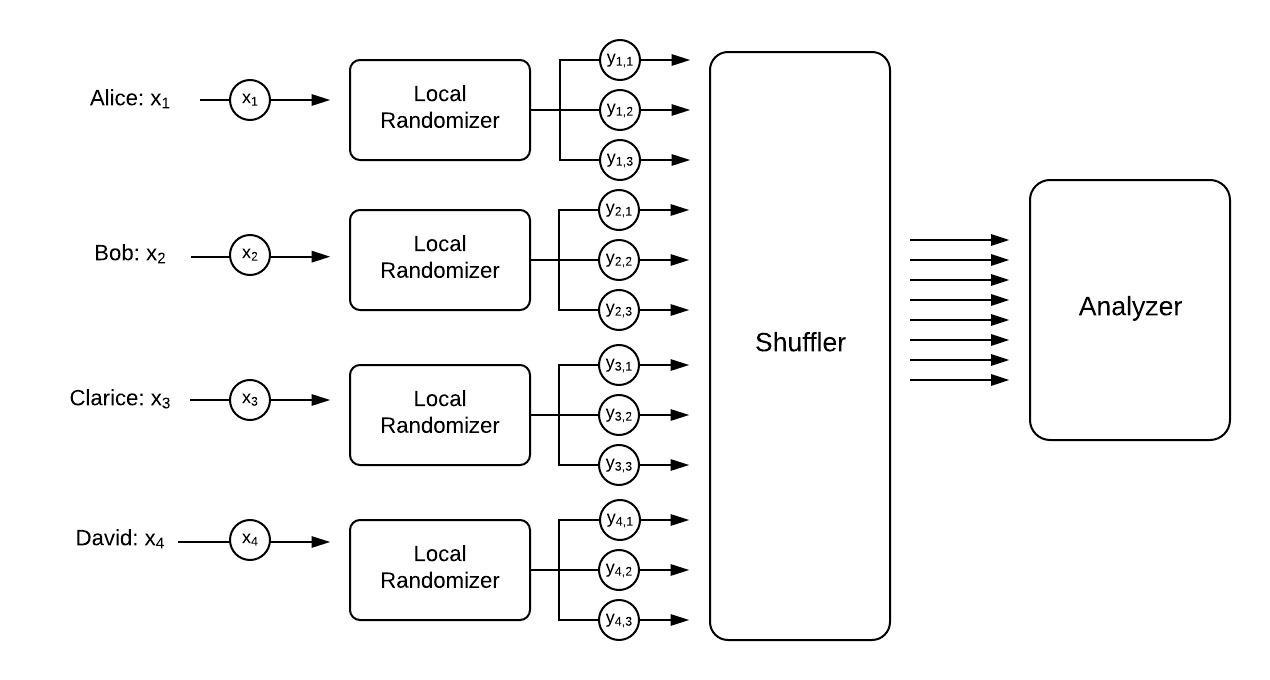
\includegraphics[width=0.7\textwidth]{esa_diagram.jpeg}
\caption{The Encode-Shuffle-Analyze (ESA) framework, illustrated here for $4$ players.}
\label{fig:esa}
\end{figure}

\citet{prochlo} proposed the Prochlo system as a way to implement the ESA framework. The system takes a holistic approach to privacy that takes into account secure computation aspects (addressed using TEEs), private disclosure aspects (addressed by means of differential privacy), and verifiability aspects (mitigated using secure enclave attestation capabilities). 

More generally, shuffling models of differential privacy can use broader classes of local randomizers, and can even select these local randomizers adaptively~\cite{erlingsson2019amplification}. This can enable differentially private protocols with far smaller error than what is possible in the local model, while relying on weaker trust assumptions than in the central model, e.g., ~\cite{cheu2019distributed, erlingsson2019amplification,BalleBGN19, ghazi2019scalable_1, ghazi2019scalable, ghazi2019private, pure-dp-shuffled, counting_shuffle_ICML, chen2020distributed}. 

% TODO(kairouz) or TODO(mcmahan): We probably needs some discussion of amplification by sampling/shuffling here, in particular the challenge for secagg that the server implementing secagg still knows which clients connected, so you get different guarantees for the server vs. say the engineer/analys who does not have this information.

\paragraph{Hybrid differential privacy}  Another promising approach is hybrid differential privacy~\cite{avent2017blender}, which combines multiple trust models by partitioning users based on their trust model preference (e.g. trust or lack of trust in the curator). Prior to the hybrid model, there were two natural choices. The first was to use the least-trusting model, which typically provides the lowest utility, and conservatively apply it uniformly over the entire userbase. The second was to use the most-trusting model, which typically provides the highest utility, but only apply it over the most-trusting users. By allowing multiple models to coexist, hybrid model mechanisms can achieve more utility from a given userbase, compared to purely local or central DP mechanisms. For instance, \cite{avent2017blender} describes a system in which most users contribute their data in the local model of privacy, and a small fraction of users opt-in to contributing their data in the central DP model. This enables the design of a mechanism which, in some circumstances, outperforms both the conservative local DP mechanism applied across all users as well as the central DP mechanism applied only across the small fraction of opt-in users. Recent work by~\cite{beimel2019power} further demonstrates that a combination of multiple trust models can become part of a promising toolkit for designing and implementing differential privacy. This construction can be directly applied in the federated learning setting; however, the general concept of combining trust models or computational models may also inspire similar but new approaches for federated learning. 



\subsubsection{Verifiability}
\label{sssec:verifiability}

%"how do I know that you did what you promised". This is of course related with (a) for malicious security, but conceptually separate. A paragraph analogous to the coverage of HE or MPC explaining very briefly the flavours of verifiability and ZNPs, seminal papers, and existing libraries / some notion of state-of-the-art would be useful I think. Ideally we would then make that specific to the (single-server / many clients) FL setting, but that can be done later I think.

An important notion that is orthogonal to the above privacy techniques is that of verifiability. Generally speaking, verifiable computation will enable one party to prove to another party that it has executed the desired behavior on its data faithfully, without compromising the potential secrecy of the data. The concept of verifiable computation dates back to \citet{DBLP:conf/stoc/BabaiFLS91} and has been studied under various terms in the literature: checking computations~\cite{DBLP:conf/stoc/BabaiFLS91}, certified computation~\cite{DBLP:journals/siamcomp/Micali00}, delegating computations~\cite{DBLP:conf/stoc/GoldwasserKR08}, as well as verifiable computing~\cite{DBLP:conf/crypto/GennaroGP10}.

In the context of FL, verifiability can be used for two purposes. First, it would enable the server to prove to the clients that it executed the intended behavior (e.g., aggregating inputs, shuffling of the input messages, or adding noise for differential privacy) faithfully. Second, it would enable the clients to prove to the server that their inputs and behavior follow that of the protocol specification (e.g., the input belongs to a certain range, or the data is a correctly generated ciphertext).

Multiple techniques can be useful to provide verifiability: zero-knowledge proofs (ZKPs), trusted execution environments (TEEs), or remote attestation. Among these ZKPs provide formal cryptographic security guarantees based on mathematical hardness, while others make rely on assumption about the security of trusted hardware.%, or auditability.

\paragraph{Zero-knowledge proofs (ZKPs)} Zero knowledge (ZK) proofs are a cryptographic primitive that enables one party (called the
\emph{prover}) to prove statements to another party (called the \emph{verifier}), that depend on secret
information known to the prover, called witness, without revealing those secrets to the verifier. The notion of zero-knowledge was introduced in the late 1980's by \citet{DBLP:journals/siamcomp/GoldwasserMR89}. It provides a solution for the verifiability question on private data. While 
there had been a large body of work on ZK construction, the first work that brought ZKPs and verifiable computation for general functionalities in the realm of practicality was the work of ~\citet{DBLP:journals/cacm/ParnoHG016} which introduces the first optimized construction and implementation for succinct ZK. Nowadays, ZKP protocols can achieve proof sizes of hundred of bytes and verifications of the order of milliseconds regardless of the size of the statement being proved.

A ZKP has three salient properties: \emph{completeness} (if the statement is true and the prover and verifier follow the protocol, the verifier will accept the proof), \emph{soundness} (if the statement is false and the verifier follows the protocol, the verifier will refuse the proof), and \emph{zero-knowledge} (if the statement is true and the prover follows the protocol, the verifier will only learn that the statement is true and will not learn any confidential information from the interaction).

Beyond these common properties, there are different types of zero-knowledge constructions in terms of supported language for the proofs, setup requirements, prover and verifier computational efficiency, interactivity, succinctness, and underlying hardness assumptions. There are many ZK constructions that support specific classes of statements, Schnorr proofs~\cite{Schnorr:1990:EIS:111563.111628} and Sigma protocols~\cite{DamgaardSigma} are examples of such widely used protocols. While such protocols have numerous uses in specific settings, general ZK systems that can support any functionality provide a much more broadly applicable tool (including in the context of FL), and thus we focus on such constructions for the rest of the discussion.

A major distinguishing feature between different constructions is the need for \emph{trusted} setup. Some ZKPs rely on a common reference string (CRS), which is computed using secrets that should remain hidden in order to guarantee the soundness properties of the proofs. The computation of such a CRS is referred to as a trusted setup. While this requirement is a disadvantage for such systems, the existing ZKP constructions that achieve most succinct proofs and verifier's efficiency require trusted setup. 

Another significant property that affects the applicability in different scenarios is whether generating the proof requires interaction between the prover and the verifier, and here we distinguish non-interactive zero-knowledge proofs (NIZKs) that enable the prover to send a single message to the verifier and require no further communication. Often we can convert interactive to non-interactive proofs by making stronger assumptions about ideal functionality of hash functions (i.e., that hash functions behave as random oracles).

Additionally, there are different measurements for efficiency of a ZKP system one must be aware of, such as the length of the proof and the computation complexity of the prover and verifier. The ideal prover's complexity should be linear in the execution time for the evaluated functionality but many existing ZKPs introduce additional (sometimes significant) overhead for the prover. The most efficient verification complexity requires computation at least linear in the size of the inputs for the evaluated functionality, and in the setting of proofs for the work of the FL server this input size will be significant.

Succinct
non-interactive zero-knowledge proofs (SNARKs)~\cite{Bitansky:2012:ECR:2090236.2090263} are a type of ZKP that provides constant proof size and verification that depends only on the input size, linearly. These attractive efficiency properties do come at the price of stronger assumptions, which is mostly inherent, %~\cite{}, 
and trusted setup in all existing scheme. Most existing SNARK constructions leverage quadratic arithmetic programs~\cite{DBLP:conf/eurocrypt/GennaroGP013,DBLP:journals/cacm/ParnoHG016,DBLP:conf/sp/CostelloFHKKNPZ15} and are now available in open-source libraries, such as libsnark~\cite{libsnark}, and deployed in cryptocurrencies, such as Zcash~\cite{DBLP:conf/sp/Ben-SassonCG0MTV14}. Note that SNARK systems usually require overhead on the part of the prover; in particular, the prover computation needs to be superlinear in the size of the circuit for the statement being proven. Recently, \citet{DBLP:conf/crypto/XieZZPS19} presented Libra, a ZKP system that achieves linear prover complexity but with increased proof size and verification time. 

If we relax the requirements for succinctness or non-interactiveness for the construction, there is a large body of constructions that achieve a wide range of efficiency trade-offs, avoid the trusted setup requirement and use more standard cryptographic assumptions~\cite{DBLP:conf/sp/BunzBBPWM18,DBLP:conf/sp/WahbyTSTW18,Ames:2017:LLS:3133956.3134104,DBLP:conf/crypto/Ben-SassonBHR19}.

%On the other side of the spectrum, systems that are interactive have longer proofs or require more work on the verifier’s side, but achieve a lower overhead for the prover. Interactive proofs of knowledge for specific statements are widely used in cryptography, and most notably in digital signatures. For example, one of the simplest and most frequently used interactive proof of knowledge is the proof of knowledge of a discrete logarithm due to \citet{DBLP:conf/crypto/Schnorr89}.
% @Mariana: can we provide meaningful references here?
% Should we talk about MPC? 
% ~\cite{DBLP:conf/crypto/Ben-SassonBHR19}.

In the recent years, an increasing numbers of practical applications have been using non-interactive zero-knowledge proofs, primarily motivated by blockchains. Using interactive ZKP systems and NIZKs efficiently in the context of FL remains a challenging open question. In such a setting, NIZKs may enable to prove to the server properties about the client's inputs. In the setting where the verifier is the client, it will be challenging to create a trustworthy statement to verify as it involves input from other clients. Of interest in this setting, recent work enables to handle the case where the multiple verifiers have shares of the statement~\cite{DBLP:conf/crypto/BonehBCGI19}. 


\paragraph{Trusted execution environment and remote attestation} We discussed TEEs in \cref{sssec:secure_computations}, but focus here on the fact that TEEs may provide opportunities to provide verifiable computations.  Indeed, TEEs enable to attest and verify the code (binary) running in its environment.  In particular, when the verifier knows (or can reproduce) which binary should run in the secure enclaves, TEEs will be able to provide a notion of \emph{integrity} (the code execution cannot be affected, except by the inputs), and an \emph{attestation} (the TEE can prove that a specific binary is executing and what is starting state was)~\cite{subramanyan2017formal, DBLP:conf/eurosp/TramerZLHJS17}. More generally, remote attestation allows a verifier to securely measure the internal state of a remote hardware platform, and can be used to establish a static or dynamic root of trust. While TEEs enable hardware-based remote attestations, both software-based remote attestions~\cite{DBLP:series/ais/SeshadriLPDK07} and hybrid remote attestation designs~\cite{DBLP:conf/ndss/EldefrawyTFP12,DBLP:conf/eurosys/KoeberlSSV14} were proposed in the literature and enable to trade off hardware requirements for verifiability.

In a federated learning setting, TEEs and remote attestations may be particularly helpful for clients to be able to efficiently verify key functions running on the server. For example, secure aggregation or shuffling could run in TEEs and would provide differential privacy guarantees on their outputs. Therefore, the post-processing logic subsequently applied by the server on the differentially private data could run on the server and remain oblivious to the clients. Note that such a system design requires the clients to know and trust the exact code (binary) for the key functions to be applied in the enclaves. Additionally, remote attestations may enable a server to attest specific requirements from the clients involved in the FL computation, such as absence of leaks, immutability, and uninterruptability (we defer to~\cite{DBLP:conf/date/FrancillonNRT14} for an exhaustive list of minimal requirements for remote attestation). 



\subsection{Protections Against External Malicious Actors}
\label{ssec:adv_clients_analysts}

In this section, we assume the existence of a trusted server and discuss various challenges and open problems towards achieving rigorous privacy guarantees against external malicious actors (e.g. adversarial clients, adversarial analysts, adversarial devices that consume the learned model, or any combination thereof). 

As discussed in Table \ref{table:actors_and_threats}, malicious clients can inspect all messages received from the server (including the model iterates) in the rounds they participate in,  malicious analysts  can inspect sequences of model iterates from multiple training runs with different hyperparameters, and in cross-device FL, malicious devices can have either white-box or black-box access to the final model. Therefore, to give rigorous protections against external adversaries, it is important to first consider what can be learned from the intermediate iterates and final model. 

\subsubsection{Auditing the Iterates and Final Model}
\label{sssec:auditing}

To better understand what can be learned from the intermediate iterates or final model, we  propose quantifying federated learning models' susceptibility towards specific attacks.
This is a particularly interesting problem in the federated learning context. On the one hand, adversaries receive direct access to the model from the server, which widens the attack surface.
On the other hand, the server determines which specific stages of the training process the adversary will receive access to the model, and additionally controls the adversary's influence over the model at each of the stages.
 
For classic (non-federated) models of computation, understanding a model's susceptibility to attacks is an active and challenging research area~\cite{fredrikson2015model, shokri2017membership, carlini2018secret, melis2018exploiting,carlini2020extracting}.
The most common method of quantifying a model's susceptibility to an attack is to simulate the attack on the model using a proxy (auditing) dataset similar to the dataset expected in practice.
This gives an idea of what the model's \textit{expected} attack susceptibility is \textit{if} the proxy dataset is indeed similar to the eventual user data. A safer method would be to determine a worst-case upper-bound on the model's attack susceptibility. This can be approached theoretically as in~\cite{yeom2018privacy}, although this often yields loose, vacuous bounds for realistic models. Empirical approaches may be able to provide tighter bounds, but for many types of attacks and models, this endeavour may be intractable. An interesting emerging area of research in this space examines the theoretic conditions (on the audited model and attacks) under which an unsuccessful attempt to identify privacy violations by a simulated attack implies that no stronger attacks can succeed at such a task \cite{diaz2019theoretical}. However, this area is still nascent and more work needs to be done to better understand the fundamental requirements under which auditing (via simulated attacks) is sufficient.

The federated learning framework provides a unique setting not only for attacks, but also for attack quantification and defense. Specifically, due to the server's control over when each user can access and influence the model during the training process, it may be possible to design new tractable methods for quantifying a model's average-case or worst-case attack susceptibility. Such methods would enable the development of new adaptive defenses, which can be applied on-the-fly to preempt significant adversarial influence while maximizing utility.

\subsubsection{Training with Central Differential Privacy}
\label{sssec:central_dp}

To limit or eliminate the information that could be learned about an individual from the iterates (and/or final model), user-level differential privacy can be used in FL’s iterative training process \cite{abadi2016deep,mcmahan18dplm,mcmahan2018general,bhowmick2018protection}. With this technique, the server clips the $\ell_2$ norm of individual updates, aggregates the clipped updates, and then adds Gaussian noise to the aggregate. This ensures that the iterates do not overfit to any individual user’s update. To track the overall privacy budget across rounds, advanced composition theorems \cite{DRV10, kairouz2017composition} or the analytical moments accountant method developed in \cite{abadi2016deep,mironov2017renyi, mironov2019r,wang2018subsampled} can be used. The moments accountant method works particularly well with the uniformly subsampled Gaussian mechanism. For moderate privacy budgets and in the absence of a sufficiently large dataset~\cite{ramaswamy2020training}, the noise introduced by this process can lead to a large decrease in model accuracy.  Prior work has explored a number of avenues to mitigate this trade-off between privacy and accuracy, including collecting more private data~\cite{mcmahan18dplm}, designing privacy-friendly model architectures~\cite{papernot2020tempered}, or leveraging priors on the private data domain~\cite{tramer2020differentially}.

In cross-device FL, the number of training examples can vary drastically from one device to the other.
Hence, similar to recent works on user-level DP in the central model~\cite{amin2019bounding}, figuring out how to adaptively bound the contributions of users and clip the model parameters remains an interesting research direction~\cite{thakkar2019differentially, pichapati2019adaclip}. More broadly, unlike record-level DP where fundamental trade-offs between accuracy and privacy are well understood for a variety of canonical learning and estimation tasks, user-level DP is fundamentally less understood (especially when the number of contributions varies wildly across users and is not tightly bounded \textit{a priori}). Thus, more work needs to be done to better understand the fundamental trade-offs in this emerging setting of DP.  Recently, \cite{liu2020learning} made progress on this front by characterizing the trade-offs between accuracy and privacy for learning discrete distributions under user-level DP.

In addition to the above, it is important to draw a distinction between malicious clients that may be able to see (some of) the intermediate iterates during training and malicious analysts (or deployments) that can only see the final model. Even though central DP provides protections against both threat models, a careful theoretical analysis can reveal that for a specific implementation of the above Gaussian mechanism (or any other differentially private mechanism), we may get different privacy parameters for these two threat models. Naturally, we should get stronger differential privacy guarantees with respect to malicious analysts than we do with respect to malicious clients (because malicious clients may have access to far more information than malicious analysts). This ``privacy amplification via iteration'' setting has been recently studied by \citet{feldman2018privacy} for convex optimization problems. However, it is unclear whether or not the results in \cite{feldman2018privacy} can be carried over to the non-convex setting.


\paragraph{Privacy amplification for non-uniform device sampling procedures}
Providing formal $(\varepsilon, \delta)$ guarantees in the context of cross-device FL system can be particularly challenging because: (a) the set of all eligible users (i.e. underlying database) is dynamic and not known in advance, and (b) users participating in federate computations may drop out at any point in the protocol. It is therefore important to investigate and design protocols that: (1) are robust to nature’s choice (user availability and dropout), (2) are self-accounting, in that the  server  can  compute a tight $(\varepsilon, \delta)$ guarantee using only information available via the protocol, (3) rely on local participation decision (i.e. do not assume that the server knows which users are online and has the ability to sample from them), and (4) achieve good privacy-utility trade-offs. While recent works \cite{balle2020privacy, kairouz2021practical} suggest that these constraints can be simultaneously achieved, building an end-to-end protocol that works in production FL systems is still an important open problem.

\paragraph{Sources of randomness (adapted from \cite{mcmahan2018general})}
Most computational devices have access only to few sources of entropy and they tend to be very low rate (hardware interrupts, on-board sensors). It is standard---and theoretically well justified---to use the entropy to seed a cryptographically secure pseudo-random number generator (PRNG) and use the PRNG's output as needed. Robust and efficient PRNGs based on standard cryptographic primitives exist that have output rate of gigabytes per second on modern CPUs and require a seed as short as 128 bits~\citep{salmon2011parallel}. 

The output distribution of a randomized algorithm~$\mathcal{A}$ with access to a PRNG is indistinguishable from the output distribution of $\mathcal{A}$ with access to a true source of entropy \emph{as long as the distinguisher is computationally bounded}. Compare it with the guarantee of differential privacy which holds against any adversary, no matter how powerful. As such, virtually all implementations of differential privacy satisfy only (variants of) computational differential privacy introduced by~\citep{Mironov-CDP}. On the positive side, a computationally-bounded adversary cannot tell the difference, which allows us to avoid being overly pedantic about this point.

A training procedure may have multiple sources of non-determinism (e.g., dropout layers or an input of a generative model) but only those that are reflected in the privacy ledger must come from a cryptographically secure PRNG. In particular, the device sampling procedure and the additive Gaussian noise must be drawn from a cryptographically secure PRNG for the trained model to satisfy computational differential privacy. 

\paragraph{Auditing differential privacy implementations}
Privacy and security protocols are notoriously difficult to implement correctly (e.g., ~\cite{mironov2012significance, haeberlen2011differential} for differential privacy). What techniques can be used for testing FL-implementations for correctness? Since the techniques will often be deployed by organizations who may opt not to open-source code, what are the possibilities for black-box testing?  Some works~\cite{ding2019detecting,liu2019minimax,jagielski2020auditing} begin to explore this area in the context of differential privacy, but many open questions remain.

\subsubsection{Concealing the Iterates}
\label{sssec:concealing_iterates}

In typical federated learning systems, the model iterates (i.e., the newly updated versions of the model after each round of training) are assumed to be visible to multiple actors in the system, including the server and the clients that are chosen to participate in each round.  However, it may be possible to use tools from~\cref{ssec:tools_tech} to keep the iterates concealed from these actors.

To conceal the iterates from the clients, each client could run their local portion of federated learning inside a TEE providing confidentiality features (see~\cref{sssec:secure_computations}).  The server would validate that the expected federated learning code is running in the TEE (relying on the TEE's attestation and integrity features), then transmit an encrypted model iterate to the device such that it can only be decrypted inside the TEE.  Finally the model updates would be encrypted inside the TEE before being returned to the server, using keys only known inside the enclave and on the server.  Unfortunately, TEEs may not be generally available across clients, especially when those clients are end-user devices such as smartphones.  Moreover, even when TEEs are present, they may not be sufficiently powerful to support training computations, which would have to happen inside the TEE in order to protect the model iterate, and may be computationally expensive and/or require significant amounts of RAM -- though TEE capabilities are likely to improve over time, and techniques such as those presented in~\cite{tramer2018slalom} may be able to reduce the requirements on the TEE by exporting portions of the computation outside the TEE while maintaining the attestation, integrity, and confidentiality needs of the computation as a whole.

Similar protections can be achieved under the MPC model~\cite{secureml, quotient}.  For example, the server could encrypt the iterate's model parameters under a homomorphic encryption scheme before sending it to the client, using keys known only to the server. The client could then compute the encrypted model update using the homomorphic properties of the cryptosystem, without needing to decrypt the model parameters.  The encrypted model update could then be returned to the server for aggregation.  A key challenge here will be to force aggregation on the server before decryption, as otherwise the server may be able to learn a client's model update.  Another challenging open problem here is improving performance, as even state-of-the-art systems can require quite significant computational resources to complete a single round of training in a deep neural network.  Progress here could be made both by algorithmic advances as well as through the development of more efficient hardware accelerators for MPC~\cite{riazi2019heax}.

Additional challenges arise if the model iterates should also be concealed from the server.  Under the TEE model, the server portion of federated learning could run inside a TEE, with all parties (i.e., clients and analyst) verifying that the server TEE will only release the final model after the appropriate training criteria have been met.  Under the MPC model, an encryption key could protect the model iterates, with the key held by the analyst, distributed in shares among the clients, or held by a trusted third party; in this setup, the key holder(s) would be required to engage in the decryption of the model parameters, and could thereby ensure that this process happens only once.

\subsubsection{Repeated Analyses over Evolving Data}
\label{sssec:repeated_analyses}

For many applications of federated learning, the analyst wishes to analyze data that arrive in a streaming fashion, and must also provide dynamically-updated learned models that are (1) correct on the data seen thus far, and (2) accurately predict future data arrivals.  In the absence of privacy concerns, the analyst could simply re-train the learned model once new data arrive, to ensure maximum accuracy at all times.  However, since privacy guarantees degrade as additional information is published about the same data \cite{DMNS06,DRV10}, these updates must be less frequent to still preserve both privacy and accuracy of the overall analysis.

Recent advances in differential privacy for dynamic databases and time series data \cite{CKM+18,CKLT18, CKM+18b} have all assumed the existence of a trusted curator who can see raw data as they arrive online, and publish dynamically updated statistics.  An open question is how these algorithmic techniques can be extended to the federated setting, to enable private federated learning on time series data or other dynamically evolving databases.

Specific open questions include:
\begin{itemize}
    \item How should an analyst privately update an FL model in the presence of new data? Alternatively, how well would a model that was learned privately with FL on a dataset $D$ extend to a dataset $D'$ that was guaranteed to be similar to $D$ in a given closeness measure?  Since FL already occurs on samples that arrive online and does not overfit to the data it sees, it is likely that such a model would still continue to perform well on a new database $D'$.  
    This is also related to questions of robustness that are explored in Section \ref{sec:robust}.
    \item One way around the issue of privacy composition is by producing synthetic data~\cite{dwork2014algorithmic,abay2018privacy}, which can then be used indefinitely without incurring additional privacy loss.  This follows from the post-processing guarantees of differential privacy \cite{DMNS06}.  \citet{augenstein2019generative} explore the generation of synthetic data in a federated fashion.  In the dynamic data setting, synthetic data can be used repeatedly until it has become ``outdated'' with respect to new data, and must be updated.  Even after generating data in a federated fashion, it must also be updated privately and federatedly.
    \item Can the specific approaches in prior work on differential privacy for dynamic databases \cite{CKLT18} or privately detecting changes in time series data \cite{CKM+18, CKM+18b} be extended to the federated setting?
    \item How can time series data be queried in a federated model in the first place?  By design, the same users are not regularly queried multiple times for updated data points, so it is difficult to collect true within-subject estimates of an individuals' data evolution over time. Common tools for statistical sampling of time series data may be brought to bear here, but must be used in conjunction with tools for privacy and tools for federation.  Other approaches include reformulating the queries such that each within-subject subquery can be answered entirely on device.
\end{itemize}

\subsubsection{Preventing Model Theft and Misuse}
\label{sssec:model_theft}

In some cases, the actor or organization developing an ML model may be motivated to restrict the ability to inspect, misuse or steal the model.  For example, restricting access to the model's parameters may make it more difficult for an adversary to search for vulnerabilities, such as inputs that produce unanticipated model outputs.  

Protecting a deployed model during inference is closely related to the challenge of concealing the model iterates from clients during training, as discussed in~\cref{sssec:concealing_iterates}.  Again, both TEEs and MPC may be used.  Under the TEE model, the model parameters are only accessible to a TEE on the device, as in~\cref{sssec:concealing_iterates}; the primary difference being that the desired calculation is now inference instead of training.  

It is harder to adapt MPC strategies to this use case without forgoing the advantages offered by on-device inference: if the user data, model parameters, and inference results are all intended to be on-device, then it is unclear what additional party is participating in the multi-party computation.  For example, na\"ively attempting to use homomorphic encryption would require the decryption keys to be on device where the inferences are to be used, thereby undermining the value of the encryption in the first place.  Solutions where the analyst is required to participate (e.g. holding either the encryption keys or the model parameters themselves) imply additional inference latency, bandwidth costs, and connectivity requirements for the end user (e.g. the inferences would no longer be available for a device in airplane mode).

It is crucial to note that even if the model parameters themselves are successfully hidden, research has shown that in many cases they can be reconstructed by an adversary who only has access to an inference/prediction API based on those parameters~\cite{DBLP:conf/uss/TramerZJRR16}.  It is an open question what additional protections would need to be put into place to protect from these kinds of issues in the context of a model residing on millions or billions of end user devices.

\subsection{Protections Against an Adversarial Server}
\label{ssec:adv_server}

In the previous section, we assumed the existence of a trusted server that can orchestrate the training process. In this section we discuss the more desirable scenario of protecting against an adversarial server. In particular, we start by investigating the challenges of this setting and existing works, and then move on to describing the open problems and how the techniques discussed in Section \ref{ssec:tools_tech} can be used to address these challenges.

\subsubsection{Challenges: Communication Channels, Sybil Attacks, and Selection}
\label{sssec:challenges}

In the cross-device FL setting, we have a server with significant computational resources and a large number of clients that (i) can only communicate with the server (as in a star network topology), and (ii) may be limited in connectivity and bandwidth. This poses very concrete requirements when enforcing a given trust model. In particular, clients do not have a clear way of establishing secure channels among themselves independent of the server. This suggests, as shown by \citet{hatelove} for practical settings, that assuming honest (or at least semi-honest) behaviour by the server in a key distribution phase (as done in~\cite{bonawitz17secagg, bell20secagg}) is required in scenarios where private channels among clients are needed. This includes cryptographic solutions based on MPC techniques. An alternative to this assumption would be incorporating an additional party or a public bulletin board (see, e.g.,~\cite{DBLP:conf/sosp/RothNFH19}) into the model that is known to the clients and trusted to not collude with the server. 

Beyond trusting the server to facilitate private communication channels, the participants in cross-device FL must also trust the server to form cohorts of clients in a fair and honest manner.  An actively malicious adversary controlling the server could simulate a large number of fake client devices (a ``Sybil attack''~\cite{sybil-attack}) or could preferentially select previously compromised devices from the pool of available devices.   Either way, the adversary could control far more participants in a round of FL than would be expected simply from a base rate of adversarial devices in the population.  This would make it far easier to break the common assumption in MPC that at least a certain fraction of the devices are honest, thereby undermining the security of the protocol. Even if the security of protocol itself remains intact (for example, if its security is rooted in a different source of trust, such as a secure enclave), there is a risk that if a large number of adversarial clients' model updates are known to or controlled by the adversary, then the privacy of the remaining clients' updates may be undermined.  Note that these concerns can also apply in the context of TEEs.  For example, a TEE-based shuffler can also be subject to a Sybil attack; if a single honest user's input is shuffled with known inputs from fake users, it will be straight forward for the adversary to identify the honest user's value in the shuffled output.

Note that in some cases, it may be possible to establish proof among the clients in a round that they are all executing the correct protocol, such as if secure enclaves are available on client devices and the clients are able to remotely attest one another.  In these cases, it may be possible to establish privacy for all honest participants in the round (e.g., by attesting that secure multi-party computation protocols were followed accurately, that distributed differential privacy contributions were added secretly and correctly, etc.) even if the model updates themselves are known to or controlled by the adversary.

\subsubsection{Limitations of Existing Solutions}
\label{sssec:limitations}
Given that the goal of FL is for the server to construct a model of the population-level patterns in the clients' data, a natural privacy goal is to quantify, and provably limit, the server's ability to reconstruct an individual client's input data. This involves formally defining (a) what is the view of the clients data revealed to the server as a result of an FL execution, and (b) what is the privacy leakage of such a view. In FL, we are particularly interested in guaranteeing that the server can aggregate reports from the clients, while somehow masking the contributions of each individual client. As discussed in Section \ref{sssec:private_disclosures}, this can be done in a variety of ways, typically using some notion of differential privacy. There are a wide variety of such methods, each with their own weaknesses, especially in FL. For example, as already discussed, central DP suffers from the need to have access to a trusted central server. This has led to other promising private disclosure methods discussed in Section \ref{sssec:private_disclosures}. Here, we outline some of the weaknesses of these methods.

\paragraph{Local differential privacy} 

As previously discussed, LDP removes the need for a trusted central server by having each client perform a differentially private transformation to their report before sending it to the central server. LDP assumes that a user's privacy comes solely from that user's addition of their own randomness; thus, a user's privacy guarantee is independent of the additional randomness incorporated by all other users.
While LDP protocols are effective at enforcing privacy and have theoretical justifications~\cite{rappor:15, applewhitepaper:17,  collecting-telemetry-data-privately}, a number of results have shown that achieving local differential privacy while preserving utility is challenging, especially in high-dimensional data settings~\cite{KLNRS11,Ullman18,kairouz2014extremal, bassily2017practical, kairouz2016discrete, ye2018optimal,duchi2013local, cormode2018marginal}.
Part of this difficulty is attributed to the fact that the magnitude of the random noise introduced must be comparable to the magnitude of the signal in the data, which may require combining reports between clients. Therefore, obtaining utility with LDP comparable to that in the central setting requires a relatively larger userbase or larger choice of $\varepsilon$ parameter~\cite{appleepsilon}.

\paragraph{Hybrid differential privacy} 

The hybrid model for differential privacy can help reduce the size of the required userbase by partitioning users based on their trust preferences. However, it is unclear which application areas and algorithms can best utilize hybrid trust model data~\cite{avent2017blender}. Furthermore, current work on the hybrid model typically assumes that regardless of the user trust preference, their data comes from the same distribution~\cite{avent2017blender, dubey2018hybrid, beimel2019power}. Relaxing this assumption is critical for FL in particular, as the relationship between the trust preference and actual user data may be non-trivial.

\paragraph{The shuffle model} 

The shuffle model enables users' locally-added noise to be amplified through a shuffling intermediary, although it comes with two drawbacks of its own.
The first is the requirement of a trusted intermediary; if users are already not trusting of the curator, then it may be unlikely that they will trust an intermediary approved of or created by the curator (though TEEs might help to bridge this gap).  The Prochlo framework~\cite{prochlo} is (to the best of our knowledge) the only existing instance.
The second drawback is that the shuffle model's differential privacy guarantee degrades in proportion to the number of adversarial users participating in the computation~\cite{BalleBGN19}.
Since this number isn't known to the users or the curator, it introduces uncertainty into the true level of privacy that users are receiving.
This risk is particularly important in the context of federated learning, since users (who are potentially adversarial) are a key component in the computational pipeline.
Secure multi-party computation, in addition to adding significant computation and communication overhead to each user, also does not address this risk when users are adding their own noise locally.


\paragraph{Secure aggregation} 

The Secure Aggregation protocols from~\cite{bonawitz17secagg, bell20secagg} have strong privacy guarantees when aggregating client reports. Moreover, the protocols are tailored to the setting of federated learning. For example, they are robust to clients dropping out during the execution (a common feature of cross-device FL) and scale to a large number of parties (up to billions for~\citet{bell20secagg}) and vector lengths. However, this approach has several limitations: (a) it assumes a semi-honest server (only in the private key infrastructure phase), (b) it allows the server to see the per-round aggregates (which may still leak information), (c) it is not efficient for sparse vector aggregation, and (d) it lacks the ability to enforce well-formedness of client inputs.  It is an open question how to construct an efficient and robust secure aggregation protocol that addresses all of these challenges.


% Next, instead of focusing on a specific threat model, in Sections~\ref{sec:adv-server} and ~\ref{sec:adv-clients} we discuss generally difficulties that arise when withstanding adversarial servers and clients, and identify research directions.

\subsubsection{Training with Distributed Differential Privacy}
\label{sssec:distributed_dp}
In the absence of a trusted server, distributed differential privacy (presented in \cref{sssec:private_disclosures}) can be used to protect the privacy of participants. 

\paragraph{Communication, privacy, and accuracy trade-offs under distributed DP} 
We point out that in distributed differential privacy three performance metrics are of general interest: accuracy, privacy and communication, and an important goal is nailing down the possible trade-offs between these parameters. We note that in the absence of the privacy requirement, the trade-offs between communication and accuracy have been well-studied in the literature on distributed estimation (e.g., \cite{suresh2017distributed}) and communication complexity (see \cite{Kushilevitz_Nisan_cc} for a textbook reference). On the other hand, in the centralized setup where all the users' data is already assumed to be held by a single entity and hence no communication is required, trade-offs between accuracy and privacy have been extensively studied in central DP starting with the foundational work of \cite{DMNS06,dwork2006our}. More recently, the optimal trade-offs between privacy, communication complexity and accuracy in distributed estimation with local DP have been characterized in \cite{ChenKO2020}, which shows that with careful encoding joint privacy and communication constraints can yield a performance that matches the optimal accuracy achievable under either constraint alone.

我们指出,在分布式差分隐私中,三个性能指标是人们普遍感兴趣的:准确性、隐私性和通信,一个重要的目标是确定这些参数之间可能的权衡。我们注意到,在没有隐私要求的情况下,关于分布式估计(例如,\cite{suresh2017distributed})和通信复杂性的文献(参见教科书参考资料\cite{Kushilevitz_Nisan_cc})对通信和准确性之间的权衡进行了很好的研究。另一方面,在集中式设置中,假设所有用户的数据都由一个实体持有,因此不需要通信,中央DP从基础工作\cite{DMNS06,dwork2006our} 开始广泛研究了准确性和隐私之间的权衡。最近,在\cite{ChenKO2020}中描述了使用局部DP的分布式估计中隐私、通信复杂性和准确性之间的最佳权衡,这表明,通过仔细编码,联邦隐私和通信约束可以产生与单独在任一约束下可实现的最佳精度相匹配的性能。

\subparagraph{Trade-offs for secure shuffling} These trade-offs have been recently studied in the shuffled model for the two basic tasks of \emph{aggregation} (where the goal is to compute the sum of the users' inputs) and \emph{frequency estimation} (where the inputs belong to a discrete set and the goal is to approximate the number of users holding a given element). See Tables~\ref{table:aggregation_shuffled_comparison} and~\ref{table:frequency_estimation_results} for a summary of the state-of-the-art for these two problems. Two notable open questions are (i) to study \emph{pure} differential privacy in the shuffled model, and (ii) to determine the optimal privacy, accuracy and communication trade-off for \emph{variable selection} in the multi-message setup (a nearly tight lower bound in the single-message case was recently obtained in \cite{ghazi2019private}).

In the context of federated optimization under the shuffled model of DP, the recent work of \cite{girgis2020shuffled} shows that multi-message shuffling is not needed to achieve central DP accuracy with low communication cost. However, it is unclear if the schemes presented achieve the (order) optimal communication, accuracy, tradeoffs.  
%% EDITOR: Disagree with the following statement; it conflates the "shuffled model" with the implementation of a secure shuffler/aggregator.  Secure shufflers and secure aggregators implemented via a TEE or a trusted third party generally tolerate arbitrary numbers of dropouts (though note that uses cases for both shuffling and aggregation often require at least a minimum number of users to be shuffled/aggregated in a cohort in order to achieve privacy goals; if too many users drop out to satisfy the privacy goals, well designed shufflers/aggregators should abort).  In the MPC model, secure aggregation protocols can tolerate a significant fraction of users dropping out, though there are upper bounds on this fraction in known protocols; shuffling has been less well studied in the MPC model, but would presumably have similar properties.
% We note that known protocols in the shuffled model are all robust to user dropout (which is one of the advantages of secure shuffling over the aforementioned secure aggregation approach). An interesting future direction is to try to make these protocols robust to the loss of a certain fraction of messages as well.

\begin{table}[t]
    \centering
    \footnotesize
    % \bgroup
    \def\arraystretch{1.75}
    \begin{tabular}{@{}lccc@{}}
        \toprule
        {\bf Reference} & 
        {\bf \#messages / $n$} & 
        {\bf Message size} & 
        {\bf Expected error}\\
        \midrule
        %\hline
        %\hline
        \cite{cheu2019distributed} & 
        $\varepsilon\sqrt{n}$
        & 1 
        & $\frac{1}{\varepsilon} \log\frac{n}{\delta}$
        \\
        \cite{cheu2019distributed}
        & $\ell$
        & 1 
        &
        $\sqrt{n} / \ell + \frac{1}{\varepsilon} \log\frac{1}{\delta}$
        \\
        %\hline
        \cite{BalleBGN19} & $1$ & $\log n$ & $\frac{n^{1/6}\log^{1/3}(1/\delta)}{\varepsilon^{2/3}}$\\
        %\hline
        \cite{balle2020} &
        $\log (\log n)$ &
        $\log n$ &
        $\frac{1}{\epsilon} \log(\log n )\sqrt{\log \frac{1}{\delta}}$ \\        
        \cite{ghazi2019scalable_1} &
        $\log(\frac{n}{\varepsilon \delta})$ & $\log(\frac{n}{\delta})$ & $\frac{1}{\varepsilon} \sqrt{\log\frac{1}{\delta}}$\\ 
        %\hline
        \cite{balle2020} &
        $\log(\frac{n}{\delta})$ & $\log n$ & $\frac{1}{\varepsilon}$\\         
        %\hline 
        \cite{ghazi2019scalable} \& \cite{balle2020} & $1 + \frac{\log(1/\delta)}{\log n}$ & $\log n$ & $\frac{1}{\varepsilon}$ \\
        \bottomrule
    \end{tabular}
    \caption{Comparison of differentially private \emph{aggregation} protocols in the multi-message shuffled model with $(\varepsilon,\delta)$-differential privacy. 
    The number of parties is $n$, and $\ell$ is an integer parameter.
    Message sizes are in bits. For readability, we assume that $\varepsilon \leq O(1)$, and asymptotic notations are suppressed.
    }
    \label{table:aggregation_shuffled_comparison}
\end{table}

\begin{table}[t]
    \centering
    \footnotesize
%\begin{adjustbox}{center}
\begin{tabularx}{\textwidth}{@{}Xcccccc@{}}
\toprule
          & \multicolumn{2}{l}{\bf \thead{Local}} & {\bf \thead{Local + shuffle}} & {\bf \thead{Shuffled,\\ single-message}} & {\bf \thead{Shuffled,\\ multi-message}} & {\bf \thead{Central}}\\
         \midrule
         Expected max. error & $\tilde{O}(\sqrt{n})$ & $\tilde{\Omega}(\sqrt{n})$ & $\tilde{O}(\min(\sqrt[4]{n}, \sqrt B))$ & $\tilde{\Omega}( \min(\sqrt[4]{n}, \sqrt{B}))$ & $\tilde{\Theta}(1)$ & $\tilde{\Theta}(1)$\\
         %\hline
         Communication/user & $\Theta(1)$ & any & $\tilde{\Theta}(1)$ & any & $\tilde{\Theta}(1)$ & $\tilde{\Theta}(1)$\\
       %\hline
      References & \cite{bassily2017practical} & \cite{bassily2015local} &~\cite{Warner65,erlingsson2019amplification,BalleBGN19} & \cite{ghazi2019private} & \cite{ghazi2019private} &~\cite{mcsherry2007mechanism,steinke2017tight}\\
    \bottomrule
    \end{tabularx}
%    \end{adjustbox}
     \caption{Upper and lower bounds on the expected maximum error for \emph{frequency estimation} on domains of size $B$ and over $n$ users in different models of DP. The bounds are stated for fixed, positive privacy parameters $\varepsilon$ and $\delta$, and $\tilde{\Theta}/\tilde{O}/\tilde{\Omega}$ asymptotic notation suppresses factors that are polylogarithmic in $B$ and $n$. The communication per user is in terms of the total number of bits sent. In all upper bounds, the protocol is symmetric with respect to the users, and no public randomness is needed. References are to the first results we are aware of that imply the stated bounds. 
     }
    \label{table:frequency_estimation_results}
  \end{table}

\subparagraph{Trade-offs for secure aggregation} It would be very interesting to investigate the following similar question for secure aggregation. Consider an FL round with $n$ users and assume that user $i$ holds a value $x_i$. User $i$ applies an algorithm $\mathcal{A}(\cdot)$ to $x_i$ to obtain $y_i = \mathcal{A}(x_i)$; here, $\mathcal{A}(\cdot)$ can be thought of as both a compression and privatization scheme. Using secure aggregation as a black box, the service provider observes $\bar{y} = \sum_i \mathcal{A}(x_i)$ and uses $\bar{y}$ to estimate $\bar{x}$, the true sum of the $x_i$'s, by computing $\hat{\bar{x}} = g(\bar{y}$) for some function $g(\cdot)$. Ideally, we would like to design $\mathcal{A}(\cdot)$, $g(\cdot)$ in a way that minimizes the error in estimating $\bar{x}$; formally, we would like to solve the optimization problem $\min_{g,\mathcal{A}} \|g(\sum_i \mathcal{A}(x_i)) - \sum_i x_i\|$, where $\|.\|$ can be either the $\ell_1$ or $\ell_2$ norm. Of course, without enforcing any constraints on $g(.)$ and $\mathcal{A}(\cdot)$, we can always choose them to be the identity function and get $0$ error. However, $\mathcal{A}(\cdot)$ has to satisfy two constraints: (1) $\mathcal{A}(\cdot)$ should output $B$ bits (which can be thought of as the communication cost per user), and (2) $\bar{y} = \sum_i \mathcal{A}(x_i)$ should be an $(\varepsilon, \delta)$-DP version of $\bar{x} = \sum_i x_i$. Thus, the fundamental problem of interest is to identify the optimal algorithm $\mathcal{A}$ that achieves DP upon aggregation while also satisfying a fixed communication budget. Looking at the problem differently, for a fixed $n$, $B$, $\varepsilon$, and $\delta$, what is the smallest $\ell_1$ or $\ell_2$ error that we can hope to achieve? We note that the work of \citet{agarwal2018cpsgd} provides one candidate algorithm $\mathcal{A}$ based on uniform quantization and binomial noise addition. Yet another solution was recently presented in \cite{kairouz2021distributed} which involves rotating, scaling, and discretizing the data, then adding discrete Gaussian noise before performing modular clipping and secure aggregation. While the sum of independent discrete Gaussians is not a discrete Gaussian, the authors show that it is close enough and present tight DP guarantees and experimental results, demonstrating that their solution is able to achieve a comparable accuracy to central DP via continuous Gaussian noise with 16 (or less) bits of precision per value. However, it is unclear if this approach achieves the optimal communication, privacy, and accuracy tradeoffs. Therefore, it is of fundamental interest to derive lower bounds and matching upper bounds on the $\ell_1$ or $\ell_2$ error under the above constraints.

\paragraph{Privacy accounting} In the central model of DP, the subsampled Gaussian mechanism is often used to achieve DP, and the privacy budget is tightly tracked across rounds of FL using the moments accountant method (see discussion in \cref{ssec:adv_clients_analysts}). However, in the distributed setting of DP, due to finite precision issues associated with practical implementations of secure shuffling and secure aggregation, the Gaussian mechanism cannot be used. Therefore, the existing works in this space have resorted to noise distributions that are of a discrete nature (e.g. adding Bernoulli or binomial noise). While such distributions help in addressing the finite precision constraints imposed by the underlying implementation of secure shuffling/aggregation, they do not naturally benefit from the moments accountant method. Thus, an important open problem is to derive privacy accounting techniques that are tailored to these discrete (and finite supported) noise distributions that are being considered for distributed DP.

\paragraph{Handling client dropouts.} The above model of distributed DP assumes that participating clients remain connected to the server during a round. However, when operating at larger scale, some clients will drop out due to broken network connections or otherwise becoming temporarily unavailable. This requires the distributed noise generation mechanism to be robust against such dropouts and also affects scaling federated learning and analytics to larger numbers of participating clients.

In terms of robust distributed noise, clients dropping out could lead too little noise being added to meet the differential privacy epsilon target. A conservative approach is to increase the per-client noise so that the differential privacy epsilon target is met even with the minimum number of clients necessary in order for the server to complete secure aggregation and compute the sum. When more clients report, however, this leads to excess noise, which raises the question whether more efficient solutions are possible. 

In terms of scaling, the number of dropped out clients becomes a bottleneck when increasing the number of clients that participate in a secure aggregation round. It may also be challenging to gather enough clients at the same time. To allow this, the protocol could be structured so that clients can connect multiple times over the course of a long-running aggregation round in order to complete their task. More generally, the problem of operating at scale when clients are likely to be intermittently available has not been systematically addressed yet in the literature.


%% EDITOR: The below is not specific to FL, so it should be in the Tools and Technologies section instead.
%% Much of this is already covered there.

%\paragraph{Shufflers}
%Implementing the shuffle model of differential privacy in the absence of a trusted party is a challenging task. The Prochlo~\cite{prochlo} is the only existing instance. However, there is a rich literature on anonymous communication, and techniques like onion routing that can may be leveraged for efficient secure shuffling without relying on an additional party besides the FL server.

%{\em Relying on an external party}
% For example,
% % Rasmus Pagh and Badhi Ghazi
% assume an \emph{honest but curious} setting where:
% \begin{itemize}
%     \item the shuffler faithfully follows the protocol and does not collude with the analyzer, and
%     \item a curious eavesdropper seeing all communication to and from the shuffler should not be able to learn anything.
% \end{itemize}
% A simple implementation of a shuffler works by double-encrypting all messages sent to the shuffler. The outer layer of encryption can be removed by the shuffler before permuting and sending the messages on to the analyzer.
% The analyzer can remove the inner layer of the encryption, revealing the set of messages but not the origin of each message.
% It is an interesting problem whether shuffling can be done with weaker assumptions without significantly increasing the round or communication complexity.



%\paragraph{Auditing distributed differential privacy implementations} 
%\todo{adriag@: what are the guarantees for a client that the code they are executing does add appropriate noise, specifically if it is shipped to the server}


\paragraph{New trust models} 
The federated learning framework motivates the development of new, more refined trust models than those previously used, taking advantage of federated learning's unique computational model, and perhaps placing realistic assumptions on the capabilities of adversarial users. 
For example, what is a reasonable fraction of clients to assume might be compromised by an adversary?  Is it likely for an adversary to be able to compromise both the server and a large number of devices, or is it typically sufficient to assume that the adversary can only compromise one or the other?  In federated learning, the server is often operated by a well-known entity, such a long-living organization.  Can this be leveraged to enact a trust model where the server's behavior is trusted-but-verified, i.e. wherein the server is not prevented from deviating from the desired protocol, but is extremely likely to be detected if it does (thereby damaging the trust, reputation, and potentially financial or legal status of the hosting organization)?

%For example, by assuming standard cryptographic constraints on the users/adversaries, can ideas from secure multi-party computation be combined with concepts from the shuffle model to enable privacy amplification of locally-added noise with provably-minimal adversarial influence \textit{without} using a trusted intermediary?

%% EDITOR: I believe this is already covered by the cross-silo discussion in ~\cref{ssec:cross-silo}.
% Another alternative trust model is that of the \emph{semi-trusted curator model}, which combines tools from differential privacy and secure encryption, and requires a trust model that lives between the centralized and local models of differential privacy.  In this model, there exist several semi-trusted curators, each of which are trusted by a small fraction of the population.  Individuals share their data with a semi-trusted curator of their choice, and the semi-trusted curators will communicate with each other to compute a function of the global data set (held distributedly across the enclaves) using a combination of differential privacy, MPC, or homomorphic encryption.  
% % Ideally, this model could combine the accuracy guarantees of the centralized model of differential privacy, with local-like privacy guarantees that an individual's data will not be shared beyond the server that they individually trust.
% Applications could include sharing medical data for research purposes, where each patient trusts their preferred hospital to see their true data, but does not want raw data shared with other hospitals. More research is needed to better understand the power of algorithmic approaches in this model, and information theoretic limitations.

\subsubsection{Preserving Privacy While Training Sub-Models}
\label{sssec:training_submodels}

Many scenarios arise in which each client may have local data that is only relevant to a relatively small portion of the full model being trained.  For example, models that operate over large inventories, including natural language models (operating over an inventory of words) or content ranking models (operating over an inventory of content), frequently use an embedding lookup table as the first layer of the neural network.  Often, clients only interact with a tiny fraction of the inventory items, and under many training strategies, the only embedding vectors for which a client's data supports updates are those corresponding to the items with which the client interacted.

As another example, multi-task learning strategies can be effective approaches to personalization, but may give rise to compound models wherein any particular client only uses the submodel that is associated with that client's cluster of users, as described in~\cref{sss:multitask-learning}.

If communication efficiency is not a concern, then sub-model training looks just like standard federated learning: clients would download the full model when they participate, make use of the sub-model relevant to them, then submit a model update spanning the entire set of model parameters (i.e. with zeroes everywhere except in the entries corresponding to the relevant sub-model).  However, when deploying federated learning, communication efficiency is often a significant concern, leading to the question of whether we can achieve communication-efficient sub-model training.

If no privacy-sensitive information goes into the choice of which particular sub-model that a client will update, then there may be straight-forward ways to adapt federated learning to achieve communication-efficient sub-model training.  For example, one could run multiple copies of the federated learning procedure, one per submodel, either in parallel (e.g. clients choose the appropriate federated learning instance to participate in, based on the sub-model they wish to update), in sequence (e.g. for each round of FL, the server advertises which submodel will be updated), or in a hybrid of the two.  However, while this approach is communication efficient, the server gets to observe which submodel a client selects.

Is it possible to achieve communication-efficient sub-model federated learning while also keeping the client's sub-model choice private?  One promising approach is to use PIR for private sub-model download, while aggregating model updates using a variant of secure aggregation optimized for sparse vectors~\cite{Chang2019OnTU,Jia2019OnTC,niu2019secure}.

Open problems in this area include characterizing the sparsity regimes associated with sub-model training problems of practical interest and developing of sparse secure aggregation techniques that are communication efficient in these sparsity regimes.  It is also an open question whether private information retrieval (PIR) and secure aggregation might be co-optimized to achieve better communication efficiency than simply having each technology operate independently (e.g. by sharing some costs between the implementations of the two functionalities.)  

Some forms of local and distributed differential privacy also pose challenges here, in that noise is often added to all elements of the vector, even those that are zero; as a result, adding this noise on each client would transform an otherwise sparse model update (i.e. non-zero only on the submodel) into a dense privatized model update (non-zero almost everywhere with high probability).  It is an open question whether this tension can be resolved, i.e. whether there is a meaningful instantiation of distributed differential privacy that also maintains the sparsity of the model updates.

\subsection{User Perception}
\label{ssec:user_perception}

Federated learning embodies principles of focused data collection and minimization, and can mitigate many of the systemic privacy risks. However, as discussed above, it is important to be clear about the protections it does (and does not) provide and the technologies that can be used to provide protections against the threat models laid out in Section \ref{ssec:actors_threat_models}. While the previous sections focused on rigorous quantification of privacy against precise threat models, this section focuses on challenges around the users' perception and needs. 

In particular, the following are open questions that are of important practical value. Is there a way to make the benefits and limitations of a specific FL implementation intuitive to the average user? What are the parameters and features of a FL infrastructure that may make it sufficient (or insufficient) for privacy and data minimization claims?
%How much privacy is enough? And from whom? 
Might federated learning give users a false sense of privacy? How do we enable users to feel safe and actually be safe as they learn more about what is happening with their data? Do users value different aspects of privacy differently? What about facts that people want to protect? Would knowing these things enable us to design better mechanism? Are there ways to model people's privacy preferences well enough to decide how to set these parameters? Who gets to decide which techniques to use if there are different utility/privacy/security properties from different techniques? Just the service provider? Or also the user? Or their operating system? Their political jurisdiction? Is there a role for mechanisms like ``Privacy for the Protected (Only)'' \cite{kearns2015protected} that provide privacy guarantees for most users while allowing targeted surveillance for socitetal priorities such as counter-terrorism? Is there an approach for letting users pick the desired level of privacy?


Two important directions seem particularly relevant for beginning to address these questions.

\subsubsection{Understanding Privacy Needs for Particular Analysis Tasks}  
Many potential use-cases of FL involve complex learning tasks and high-dimensional data from users, both of which can lead to large amounts of noise being required to preserve differential privacy.  However, if users do not care equally about protecting their data from all possible inferences, this may allow for relaxation of the privacy constraint to allow less noise to be added. For example, consider the data generated by a smart home thermostat that is programmed to turn off when a house is empty, and turn on when the residents return home.  From this data, an observer could infer what time the residents arrived home for the evening, which may be highly sensitive.  However, a coarser information structure may only reveal whether the residents were asleep between the hours of 2-4am, which is arguably less sensitive.  

This approach is formalized in the Pufferfish framework of privacy \cite{pufferfish}, which allows the analyst to specify a class of protected predicates that must be learned subject to the guarantees of differential privacy, and all other predicates can be learned without differential privacy. For this approach to provide satisfactory privacy guarantees in practice, the analyst must understand the users' privacy needs to their particular analysis task and data collection procedure. The federated learning framework could be modified to allow individual users to specify what inferences they allow and disallow. These data restrictions could either be processed on device, with only ``allowable'' information being shared with the server in the FL model update step, or can be done as part of the aggregation step once data have been collected.  Further work should be done to develop technical tools for incorporating such user preferences into the FL model, and to develop techniques for meaningful preference elicitation from users.

\subsubsection{Behavioral Research to Elicit Privacy Preferences} 
Any approach to privacy that requires individual users specifying their own privacy standards should also include behavioral or field research to ensure that users can express informed preferences.  This should include both an \emph{educational component} and \emph{preference measurement}.

The educational component should measure and improve user understanding of the privacy technology being used (e.g., Section \ref{ssec:tools_tech}) and the details of data use.  For applications involving federated learning, this should also include explanations of federated learning and exactly what data will be sent to the server.  Once the educational component of the research has verified that typical users can meaningfully understand the privacy guarantees offered by a private learning process, then researchers can begin preference elicitation.  This can occur either in behavioral labs, large-scale field experiments, or small focus groups.  Care should be exercised to ensure that the individuals providing data on their preferences are both informed enough to provide high quality data and are representative of the target population.

While the rich field of behavioral and experimental economics have long shown that people behave differently in public versus private conditions (that is, when their choices are observed by others or not), very little behavioral work has been done on eliciting preferences for differential privacy \cite{CDHL19,AS19}.  Extending this line of work will be a critical step towards widespread future implementations of private federated learning. Results from the educational component will prove useful here in ensuring that study participants are fully informed and understand the decisions they are facing. It should be an important tenant of these experiments that they are performed ethically and that no deception is involved.

\subsection{Executive Summary}
\begin{itemize}
    \item Preserving the privacy of user data requires considering both {\em what} function of the data is being computed and {\em how} the computation is executed (and in particular, who can see/influence intermediate results). [Section~\ref{ssec:tools_tech}] 
    \begin{itemize}
        \item Techniques for addressing the ``{\em what}'' include data minimization and differential privacy.  [Sections~\ref{sssec:private_disclosures}, \ref{sssec:central_dp}].  It remains an important open challenge how best to adapt differential privacy accounting and privatization techniques to real world deployments, including the training of numerous machine learning models over overlapping populations, with time-evolving data, by multiple independent actors, and in the context of real-world non-determinancies such as client availability, all without rapidly depleting the privacy budget and while maintaining high utility.
        \item Techniques for addressing the ``{\em how}'' include secure multi-party computation (MPC), homomorphic encryption(HE), and trusted execution environments (TEEs).  While practical techniques MPC techniques for some federation-crucial functionalities have been deployed at scale, many important functionalities remain far more communication- and computation-expensive than their insecure counterparts.  Meanwhile, it remains an open challenge to produce a reliably exploit-immune TEE platform, and the supporting infrastructure and processes to connect attested binaries to specific privacy properties is still immature. [Section~\ref{sssec:secure_computations}]
        \item Techniques should be composed to enable {\em Privacy in Depth}, with privacy expectations degrading gracefully even if one technique/component of the system is compromised. [Section~\ref{ssec:actors_threat_models}]
        \item {\em Distributed differential privacy} best combines {\em what} and {\em how} techniques to offer high accuracy and high privacy under an honest-but-curious server, a trusted third-party, or a trusted execution environment.  [Sections~\ref{sssec:private_disclosures}, \ref{sssec:distributed_dp}]
    \end{itemize}
    \item {\em Verifiability} enables parties to prove that they have executed their parts of a computation faithfully.
    \begin{itemize}
        \item Techniques for {\em verifiability} include both zero knowledge proofs (ZKPs) and trusted execution environments (TEEs).  [Section~\ref{sssec:verifiability}]
        \item Strong protection against an adversarial server remains a significant open problem for federation. [Section~\ref{ssec:adv_server}]
    \end{itemize}
\end{itemize}